\documentclass[aspectratio=1610]{beamer}

\usepackage[ngerman]{babel}
\usepackage[utf8]{inputenc}
\usepackage[absolute,overlay]{textpos}
\usepackage{hyperref}
\usetheme{lankton-keynote}

\AtBeginSection[]
{
   \begin{frame}
       \frametitle{Outline}
       \tableofcontents[currentsection]
   \end{frame}
}

\title{Das \\„wer, wie, was, warum?“ \\der Verschlüsselung}

\author[Mic]{Mic \flq nomaster@chaosdorf.de\frq}

\institute[kunstakademie]{Kunstakademie Düsseldorf}

\date[]{15. Januar 2014}

\renewcommand{\quote}[2]
{
  \begin{exampleblock}{}
    {\large “#1”}
    \vskip5mm
    \hspace*\fill{\small--- #2}
  \end{exampleblock}
}


\begin{document}

  \begin{frame}
    \titlepage
  \end{frame}

  \begin{frame}{CryptoParty}
    \begin{itemize}
      \item Zeige den Menschen praktische Verschlüsselung
      \item Mache es unabhängig und barrierefrei
      \pause
      \item Learning by Doing
      \item Have a lot of fun
    \end{itemize}
  \end{frame}
 
  \begin{frame}{Person des Jahres 2013}
    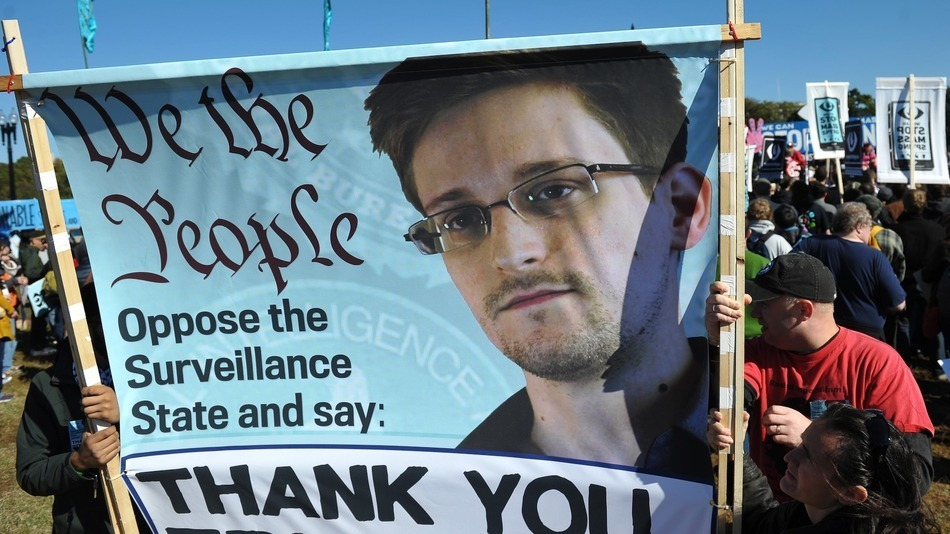
\includegraphics[width=\textwidth]{snowden.png}\\
    Edward Snowden
  \end{frame}

  \begin{frame}{Zitat}
    \quote{Man is least himself when he talks in his own person.\\
      Give him a mask, and he will tell you the truth.}
      {Oscar Wilde}
  \end{frame}

  \begin{frame}{Ohne Verschlüsselung}
    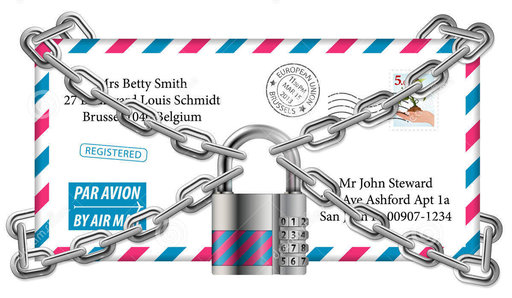
\includegraphics[width=\textwidth]{mail.jpg}
  \end{frame}

  \begin{frame}{Mit Verschlüsselung}
    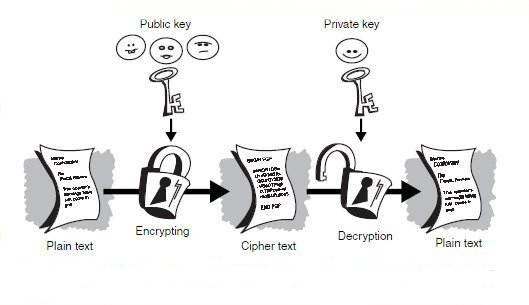
\includegraphics[width=\textwidth]{encryption.jpg}
  \end{frame}

  \begin{frame}{Privatsphäre}
    Privatsphäre ist…
    \begin{enumerate}
      \pause
      \item Der Bereich der persönlichen Freiheit
      \pause
      \item Das Recht, in Ruhe gelassen zu werden
      \pause
      \item Kontrolle über personenbezogene Daten
    \end{enumerate}
  \end{frame}

  \begin{frame}{Warum kämpfen?}
    “Ich habe doch nichts zu verbergen.”
    \pause
    \begin{itemize}
      \item Unbewusste Geheimnisse
      \item Unsichere Zukunft
      \item Auswirkungen auf andere
      \item Chilling Effect
    \end{itemize}
  \end{frame}

  \begin{frame}{Prinzip Verschlüsselung}
    \begin{columns}
      \begin{column}{.5\textwidth}
        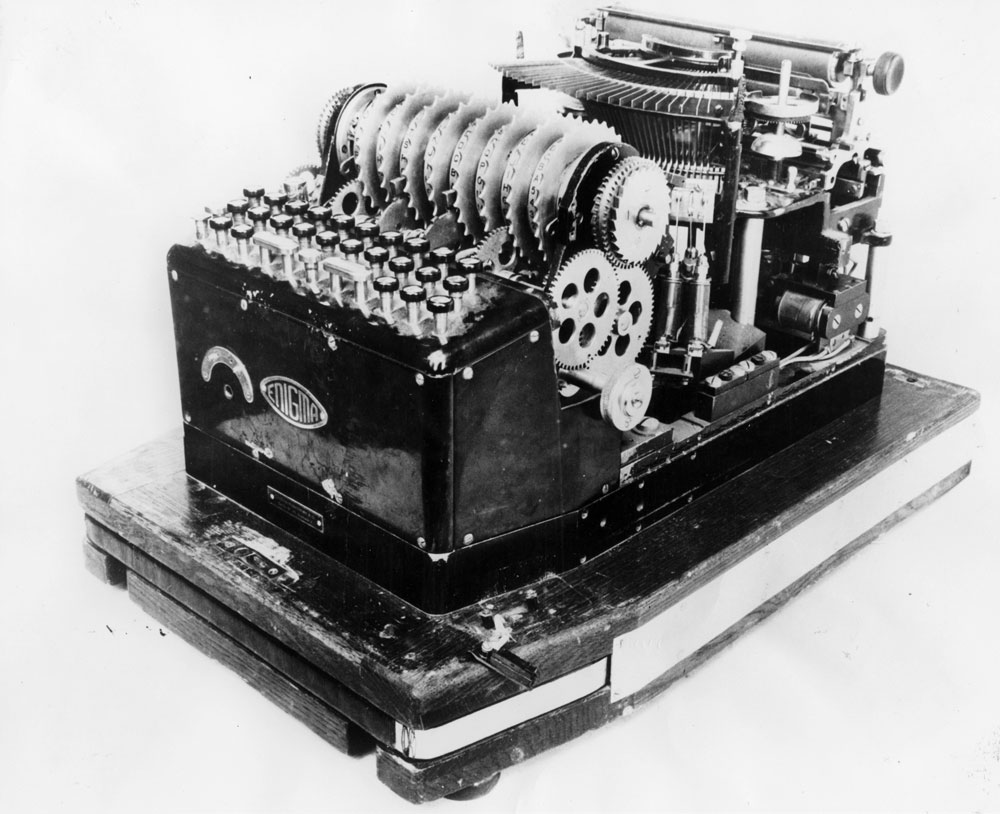
\includegraphics[width=\textwidth]{enigma.jpg}
      \end{column}
      \begin{column}{.5\textwidth}
        \begin{itemize}
          \pause
          \item Kryptographie verbirgt Informationen vor der Öffentlichkeit
          \pause
          \item Das Geheimnis muss bekannt sein
          \pause
          \item Ohne Vertrauen läuft es nicht
        \end{itemize}
      \end{column}
    \end{columns}
    \pause
    \quote{Traue niemandem!}{anonymous}
  \end{frame}

  \begin{frame}{Identität}
    \quote{Man kann nicht zweimal in den selben Fluss steigen}{panta rhei}
    \pause
    \begin{itemize}
      \item Vertrauen entsteht über die Zeit
      \item Vertrauen braucht Identität
      \item Vertrauen ist vergänglich
    \end{itemize}
  \end{frame}

  \begin{frame}{Schlüssel}
    \begin{columns}
      \begin{column}{.5\textwidth}
        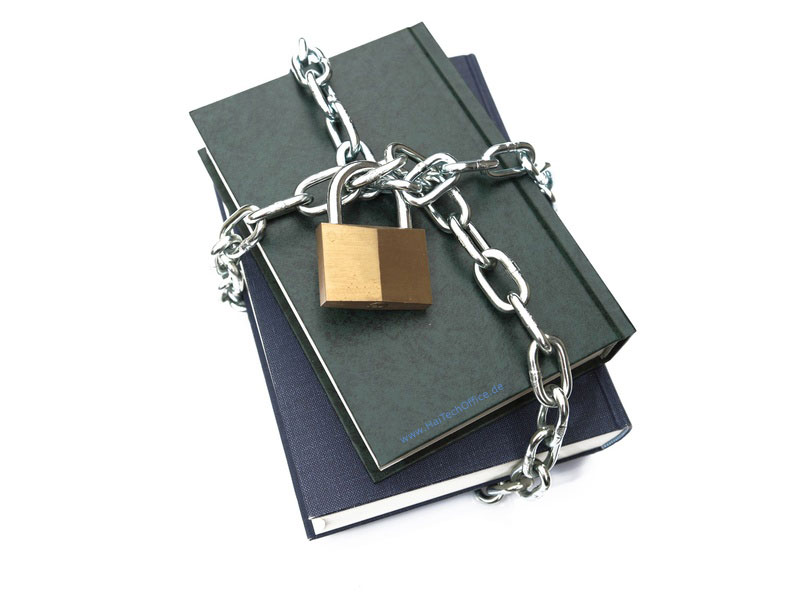
\includegraphics[width=\textwidth]{security.jpg}
      \end{column}
      \begin{column}{.5\textwidth}
        \begin{itemize}
          \item Symmetrische Schlüssel für Datenträger
          \item Asymmetrische Schlüssel für Telekommunikation
          \item Verschlüsselung ist ein Protokoll
        \end{itemize}
      \end{column}
    \end{columns}
  \end{frame}

  \begin{frame}{Meta}
    Nun kommt die Enttäuschung:
    \pause
    \begin{itemize}
      \item Verschlüsselung versteckt nur die Nachricht, nicht den Umschlag
      \item Metadaten bleiben öffentlich
    \end{itemize}
    \pause
    \begin{itemize}
      \item Identität der Sender und Empfänger
      \item Zeitpunkt und Zugangspunkt
      \item Länge und Medium
    \end{itemize}
    \pause
    \quote{Es kommt auf das Angriffsszenario an. Und es ist kompliziert.}{EFF}
  \end{frame}

  \begin{frame}{Sicherheit}
    \quote{Ein System muss auch dann sicher sein,\\wenn das gesamte System
    offen liegt:\\ausgenommen des Geheimnisses.}{Kerckhoff’sches Prinzip}
    \begin{itemize}
      \pause
      \item Die Software muss einsehbar sein.
      \pause
      \item Der Transport kann öffentlich sein.
      \pause
      \item Keine Sicherheit durch Obskurität!
    \end{itemize}
  \end{frame}

  \begin{frame}{Schlüsselwerkzeuge}
    \pause
    Verschlüsselung von Datenträgern
    \begin{itemize}
      \pause
      \item TrueCrypt
      \pause
      \item LUKS (Linux)
    \end{itemize}
    \pause
    Verschlüsselung von Nachrichten
    \begin{itemize}
      \pause
      \item Enigmail für Thunderbird
      \pause
      \item GPGTools für Apple Mail
      \paus
      \item OTR für Jabber
    \end{itemize}
    \pause
    Verschlüsselung von Verbindungen
    \begin{itemize}
      \pause
      \item OpenVPN
      \pause
      \item Tor
    \end{itemize}
  \end{frame}

  \begin{frame}{Dokumentation}
    Handbücher
    \begin{itemize}
      \pause
      \item CryptoParty Handbook \\ \url{http://www.cryptoparty.in/documentation/handbook}
      \pause
      \item Wikibooks Privacy-Handbuch \\ \url{https://de.wikibooks.org/wiki/Privacy-Handbuch}
    \end{itemize}
  \end{frame}

  \begin{frame}
    \center
    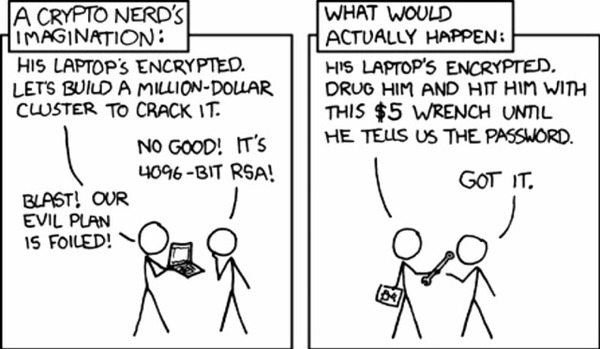
\includegraphics[width=.5\textwidth]{xkcd.jpg}
  \end{frame}

\end{document}
